Electroencephalography is an imaging technique used to record the electrical activity generated by the brain. It refers specifically to the experimental and clinical procedure by which electrical potentials are measured using electrodes placed on or within the head. Electroencephalography is widely used in both clinical neurophysiology and neuroscience research, primarily due to its ability to capture brain activity with high temporal resolution, making it particularly well suited for the study of dynamic neural processes~\cite{st-louis-2016}.

The result of this measurement technique is an electroencephalogram (also \gls{eeg}), which denotes the recorded signal itself. An \gls{eeg} consists of voltage measurements as a function of time, obtained at particular electrode locations. 

The first electroencephalographic recordings in humans were reported in 1924 by Hans Berger, who demonstrated that brain electrical activity could be measured noninvasively from the scalp~\cite{st-louis-2016}. Berger’s work established the foundations of \gls{eeg} and introduced the electroencephalogram as a meaningful representation of brain activity in humans.

From a physiological perspective, the signals observed in an electroencephalogram arise from electrical currents generated by neuronal activity. At the cellular level, synaptic activation induces the movement of ions such as Na$^+$, K$^+$, Ca$^{2+}$, and Cl$^-$ across neuronal membranes, producing local current flows. When large populations of neurons are activated in a coordinated manner, these currents sum and give rise to electric fields that can be detected as voltage differences by \gls{eeg} electrodes~\cite{abhang-2016,cherian-2024}.

The dominant contribution to electroencephalographic signals originates from synchronized postsynaptic potentials in cortical pyramidal neurons. Due to their geometry, alignment, and organization within the cerebral cortex, these neurons form effective electrical dipoles between the neuronal soma and apical dendrites, making them particularly influential in shaping the signals recorded in electroencephalograms~\cite{abhang-2016}.

\subsubsection{EEG Signal Characteristics and Spectral Bands}
Through his early experiments, Berger observed that electroencephalograms change in a \textit{consistent and recognizable manner} with the state of the subject. Transitions between conditions such as sleep, relaxation, and alertness were found to be accompanied by characteristic changes in the recorded brain activity~\cite{st-louis-2016,abhang-2016}. These observations provided the first evidence that \gls{eeg} signals exhibit structured temporal patterns related to brain state, motivating subsequent efforts to classify \gls{eeg} activity into distinct rhythmic components. One decade later, Adrian and Matthews published results consistent with Berger’s findings~\cite{abhang-2016}.

Nowadays, electroencephalographic activity is commonly described in terms of frequency bands, each associated with characteristic frequency ranges and general physiological or cognitive states. A summary of these bands is provided in Table~\ref{tab:eeg_frequency_bands}.

\begin{table}[htbp]
\centering
\caption[Commonly defined EEG frequency bands.]{Commonly defined EEG frequency bands~\cite{nayak-2025}.}
\label{tab:eeg_frequency_bands}
\begin{tabular}{lll}
\hline
\textbf{Band} & \textbf{Frequency range (Hz)} & \textbf{Related state} \\
\hline
Delta~$\delta$  & 0.5--4   & Sleep \\
Theta~$\theta$  & 4--7     & Drowsiness, early sleep; heightened emotional states \\
Alpha~$\alpha$  & 8--13    & Relaxed wakefulness, eyes closed \\
Beta~$\beta$    & 13--30   & Alertness, active thinking \\
Gamma~$\gamma$  & $>$30    & High-level cognitive processing \\
\hline
\end{tabular}
\end{table}

From a clinical perspective, \gls{eeg} analysis typically focuses on frequency components in the range of approximately 0.5 to 70~Hz, although signals are commonly
recorded up to 100~Hz~\cite{kong-2025}, with scalp-recorded potentials exhibiting relatively small amplitudes under physiological conditions, typically on the
order of 15 to 150~$\mu$V~\cite{Naydenov2022}.

Although the frequency bands summarized above are broadly associated with characteristic brain states, their interpretation is not exclusive. \gls{eeg} patterns are
influenced by multiple factors beyond the general state of the subject, including age, mental and physical condition, and pharmacological effects, which must be
considered when analyzing and interpreting \gls{eeg} recordings.

The following descriptions summarize the main characteristics of each \gls{eeg} frequency band as commonly reported in the literature~\cite{nayak-2025}.

\paragraph*{Delta rhythm}
Delta activity is the slowest \gls{eeg} rhythm and predominates during deep stages of sleep. In awake adults, prominent delta activity is uncommon and may indicate altered or pathological brain function.

\paragraph*{Theta rhythm}
Theta activity commonly appears during drowsiness and early sleep stages and is most prominent in frontal and central regions. It has also been associated with emotional processing and cognitive control, particularly in young adults.

\paragraph*{Alpha rhythm}
Alpha activity represents the dominant background rhythm of the normal adult \gls{eeg} and is most prominent over occipital regions during relaxed wakefulness. It typically attenuates with eye opening or increased cognitive engagement.

\paragraph*{Mu rhythm}
The mu rhythm ($\mu$, 8--13~Hz) occupies a frequency range similar to that of alpha activity but represents a distinct functional phenomenon. It's observed over central sensorimotor cortices and is related to motor and somatosensory processing. Unlike alpha activity, the mu rhythm is not attenuated by eye opening but is suppressed during voluntary movement, motor imagery, or observation of actions, reflecting activation of sensorimotor networks.

\paragraph*{Beta rhythm}
Beta activity is frequently observed during alert wakefulness and active mental processing. It is most prominent over frontal and central regions and may be influenced by attention and pharmacological agents.

\paragraph*{Sigma rhythm}
Sigma activity (12--16~Hz), commonly referred to as sleep spindles, is physiologically observed during non-rapid eye movement sleep, particularly stage N2. Sleep spindles reflect thalamocortical circuit activity and are considered markers of sleep-related mechanisms, including brain development, sensory information processing, and memory consolidation.

\paragraph*{Gamma rhythm}
Gamma activity is associated with higher-order cognitive functions, including attention, memory, and sensory integration. Due to its higher frequency, gamma activity is often examined in specialized clinical or research contexts.

\paragraph*{High-frequency rhythm}
High-frequency \gls{eeg} activity above 30~Hz includes gamma-band oscillations as well as higher-frequency components commonly referred to as high-frequency oscillations.
Activity above approximately 80~Hz is often subdivided into ripples and fast ripples, which are primarily observed in pathological contexts and are strongly associated
with epileptogenic tissue. These signals are typically studied in specialized clinical or invasive recording settings as they are heavily attenuated by the skull and scalp
layers, and obfuscated by muscular and ocular artifacts~\cite{FREEMAN20031053, nayak-2025}.


\subsubsection{Clinical Applications of EEG}
Electroencephalography is widely used across multiple clinical domains, including neurology, critical care, anesthesia, sleep medicine, and cognitive rehabilitation. Its applications span diagnosis, monitoring, outcome prediction, surgical planning and guidance, and even direct therapeutic intervention.

\paragraph*{Neurology}
In epilepsy diagnosis and management, \gls{eeg} remains the gold standard. It can detect nonconvulsive seizures, nonconvulsive status epilepticus, and other paroxysmal events~\cite{herman-2015}. A 2018 guideline from the International Federation of Clinical Neurophysiology highlights \gls{eeg} as \textit{essential} for diagnosing and monitoring patients with epilepsy~\cite{tatum-2018}. Routine \gls{eeg} recordings (30–60~min) are recommended, and extended monitoring up to 48~hours can increase diagnostic yield to 80–95\%. \gls{eeg} is also fundamental for localizing seizure foci, a critical step in pre-surgical evaluation~\cite{herman-2015}.

In encephalopathies—whether metabolic, toxic, degenerative, or infectious—EEG commonly reveals generalized slowing of dominant rhythms and background activity. Clinically, \gls{eeg} is first used to rule out seizures as a cause of altered mental status. Once encephalopathy is confirmed, \gls{eeg} serves to assess the degree of cerebral dysfunction. In some instances, observed patterns may suggest specific etiologies~\cite{rayi-2024}.

\paragraph*{Anesthesia and Sedation Monitoring}
\gls{eeg}-based monitors are employed to assess the depth of anesthesia and sedation. Processed \gls{eeg} indices—such as the Bispectral Index (BIS)—condense complex \gls{eeg} dynamics into a single numerical value (0–100) that correlates with levels of consciousness. Studies and clinical guidelines indicate that BIS-guided sedation may reduce the incidence of intraoperative awareness compared to standard practice. Additionally, maintaining BIS values within the 40–60 range has been associated with improved postoperative recovery, including faster emergence and reduced recovery-room duration~\cite{mathur-2023}.


\paragraph*{Sleep Medicine}
Polysomnography (\gls{psg}) integrates several physiological measurements recorded during sleep, including \gls{eeg}, electrooculogram, electrocardiogram, electromyogram, pulse oximetry, and airflow. \gls{psg} is considered the gold standard for diagnosing sleep-related breathing disorders. \gls{eeg} plays a central role in sleep staging, relying on specific waveforms—such as alpha and beta rhythms, K-complexes, and spindles—to determine the subject’s sleep phase~\cite{gerstenslager-2023,rundo-2019}.


\paragraph*{Neurorehabilitation and Neurofeedback}
In neurorehabilitation, \gls{eeg} can play a therapeutic role. \gls{eeg}-based neurofeedback, when used alongside conventional therapy, has been shown to enhance cognitive recovery~\cite{arroyo-ferrer-2021}.


\paragraph*{Brain–Computer Interfaces} 
Although still largely confined to the research domain, brain–computer interfaces constitute a promising clinical application of \gls{eeg} with the potential to significantly improve quality of life. Current applications include robotic limb or cursor control for individuals with severe motor impairments or paralysis~\cite{ding-2025}, as well as assistive communication systems for patients with speech disabilities. Beyond compensating for lost function, BCIs have also been explored as therapeutic and training tools. Notably, \gls{eeg}-based \gls{bci} videogames have been proposed to train sustained attention in children with attention deficit hyperactivity disorder, leveraging real-time neurophysiological feedback to modulate cognitive states~\cite{munoz-2015}. While many of these developments target clinical and rehabilitative settings, similar \gls{bci} principles are increasingly being investigated in non-medical and consumer-oriented contexts~\cite{varbu-2022}.

\subsubsection{EEG electrode placement systems}

Standardized electrode placement systems are used in electroencephalography to ensure anatomical consistency and reproducibility across subjects,
recording sessions, and laboratories. These systems define electrode locations as proportions of scalp distances measured between anatomical landmarks,
such as the nasion, inion, and preauricular points, thereby accommodating differences in head size and shape~\cite{klem-1999}.

The most widely adopted framework is the International 10{-}20 system, originally formalized to standardize earlier practices in clinical \gls{eeg}.
Several extensions of this system have since been introduced to increase spatial sampling density, including the 10{-}10 system and higher-resolution
schemes such as the 10{-}5 (or 5\%) system. These extensions preserve compatibility with the original 10{-}20 nomenclature, ensuring that electrode labels
remain consistent across different spatial resolutions~\cite{klem-1999}. As a result, recordings obtained with higher-density layouts can be directly related to
conventional clinical \gls{eeg} configurations.

In all these systems, electrode labels consist of a letter indicating the general cortical region—frontal~(F), temporal~(T), central~(C), parietal~(P),
and occipital~(O)—and a numerical index denoting hemispheric location. Odd numbers correspond to the left hemisphere, even numbers to the right, and the suffix \textit{z}
designates midline positions.

In this work, electrode placement follows the International 10{-}20 system, which remains the clinical standard for routine \gls{eeg} acquisition.
A conventional 10{-}20 montage typically comprises 21 electrodes, providing representative coverage of the major cortical regions while maintaining
a balance between spatial resolution and practical feasibility.

\begin{figure}[htbp]
\centering
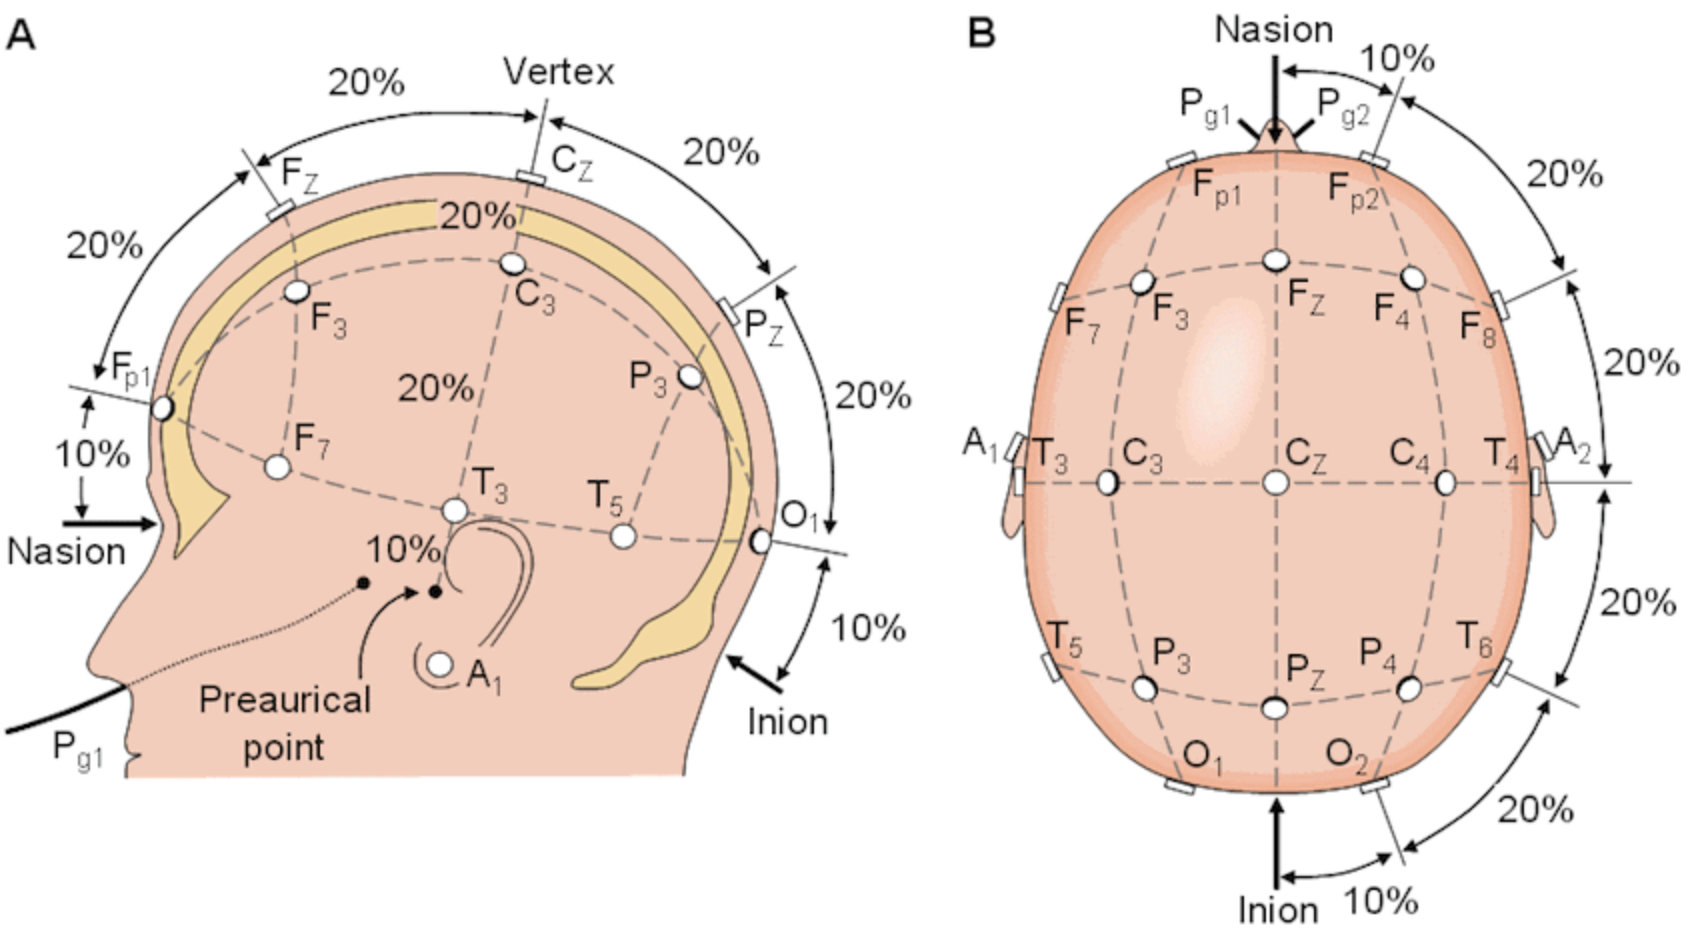
\includegraphics[width=0.5\textwidth]{../../02_Images/the-10-20-system-with-percentages.png}
\caption[EEG electrode placement systems: the 10--20 standard]{International 10{-}20 EEG electrode placement system. Image taken from~\cite{eeg-photo}.}
\label{fig:10_20_system}
\end{figure}

